\documentclass[../body.tex]{subfiles}
\begin{document}

Условия, наложенные на оптимизатор:
\\Максимальное число итераций: 50
\\Погрешность: $10^{-6}$
\\Остальные решения отбраковывались.

\subsection{Регуляризация вектора $\textbf{b}$}
Здесь введем следующую метрику: вектора $\textbf{b}$ можно интерпретировать как две точки двумерного пространства, или отрезок. Тогда за расстояние между двумя такими векторами можно принять полусумму расстояний до соответствующих концов отрезков. Можно было бы интерпретировать эти вектора как прямые, но тогда при пересечении расстояние между ними 0, что не подойдет в качестве метрики, так как в дальнейшем будет показано, что в свободной части нужно изменить только верхний интервал, причем один из его концов будет фиксированным, а второй меняться в определенных пределах.
\\$\rho$($\textbf{b}_1$, $\textbf{b}_2$) = ($\sqrt{(inf(b_1[1]) - inf(b_2[1]))^2 + (sup(b_1[1]) - sup(b_2[1]))^2}$ + 
\begin{equation}
  +\sqrt{(inf(b_1[2]) - inf(b_2[2]))^2 + (sup(b_1[2]) - sup(b_2[2]))^2})/2  \label{metric}
\end{equation}
\\ - расстояние между векторами $\textbf{b}_1$ и $\textbf{b}_2$ 


\\Теперь непосредственно к результатам.
\begin{equation}
	   \\\textrm{mid}(\textbf{b}) = \begin{pmatrix}
        0.5\\
        0.5
        \end{pmatrix}, \textrm{rad}(\textbf{b})_{opt} = \begin{pmatrix}
        2.5\\
        1.5
        \end{pmatrix}, \textbf{b}_{opt} = \begin{pmatrix}
        [-2;3]\\
        [-1;2]
        \end{pmatrix}
        \label{vec_1}
	\end{equation}
Как можно заметить, нижний интервал вошел без изменений. Получили:
\\Решение: $\textbf{x} = \begin{pmatrix}
        [0.33;0.5]\\
        [-0.5;1.67]
        \end{pmatrix}$
\\Итераций: 3
\\Погрешность (порядок): $10^{-16}$
\\Расстояние по метрике: 0.7
\\В силу малого числа итераций представим матрицу субградиента D и вектор разности dx на каждой итерации:
\\$\textrm{D}^{(1)} = \begin{pmatrix}
        3& 6& 0& 0\\
        0& 0& 0& -3\\
        0& 0& 3& 6\\
        0& -3& 0& 0
        \end{pmatrix}$, $\textrm{dx}^{(1)} = \begin{pmatrix}
        -1.09&\\
        1.33&\\
        1.04&\\
        -0.67&
        \end{pmatrix}$
\\$\textrm{D}^{(2)} = \begin{pmatrix}
        3& 6& 0& 0\\
        0& 0& -1& -3\\
        0& 0& 4& 6\\
        0& -3& 1& 0
        \end{pmatrix}$, $\textrm{dx}^{(2)} = \begin{pmatrix}
        -0.33&\\
        0.17&\\
        0.17&\\
        -0.17&
        \end{pmatrix}$
\\$\textrm{D}^{(3)} = \begin{pmatrix}
        3& 6& 0& 0\\
        0& 1& -1& 0\\
        0& 0& 4& 6\\
        0& -3& 1& 0
        \end{pmatrix}$, $\textrm{dx}^{(3)} = \begin{pmatrix}
        -0.0&\\
        0.0&\\
        0.0&\\
        -0.0&
        \end{pmatrix}$
\\Исследования $\textbf{b}_{opt}$ показали, что если оставить второй интервал без изменений, а у первого варьировать радиус в промежутке [0; 2.5], то у такой ИСЛАУ будут решения. При радиусах 2.51 и 2.501 решений уже нет. Это говорит о том, что 2.5 - это точная верхняя граница для радиусов верхнего элемента.
\\Теперь будем растягивать интервал. Получим: $\textbf{b}_{opt} =         \begin{pmatrix}
        [-3;3]\\
        [-1;2]
        \end{pmatrix}$
\\Решение: $\textbf{x} = \begin{pmatrix}
        [0.0;0.5]\\
        [-0.5;1.67]
        \end{pmatrix}$
\\Итераций: 3
\\Погрешность (порядок): $10^{-15}$
\\Расстояние по метрике: 0.5
\\В силу малого числа итераций представим матрицу субградиента D и вектор разности dx на каждой итерации:
\\$\textrm{D}^{(1)} = \begin{pmatrix}
        3& 6& 0& 0\\
        0& 0& 0& -3\\
        0& 0& 3& 6\\
        0& -3& 0& 0
        \end{pmatrix}$, $\textrm{dx}^{(1)} = \begin{pmatrix}
        -1.95&\\
        1.33&\\
        1.05&\\
        -0.67&
        \end{pmatrix}$
\\$\textrm{D}^{(2)} = \begin{pmatrix}
        3& 6& 0& 0\\
        0& 0& -1& -3\\
        0& 0& 4& 6\\
        0& -3& 1& 0
        \end{pmatrix}$, $\textrm{dx}^{(2)} = \begin{pmatrix}
        -0.33&\\
        0.17&\\
        0.17&\\
        -0.17&
        \end{pmatrix}$
\\$\textrm{D}^{(3)} = \begin{pmatrix}
        3& 6& 0& 0\\
        0& 1& -1& 0\\
        0& 0& 4& 6\\
        0& -3& 1& 0
        \end{pmatrix}$, $\textrm{dx}^{(3)} = \begin{pmatrix}
        -0.0&\\
        0.0&\\
        0.0&\\
        -0.0&
        \end{pmatrix}$
\\Заметим, что левая граница верхнего интервала совпала с исходной. При этом попытки растянуть правый интервал оказались безуспешны.
\subsection{Регуляризация матрицы $\textbf{A}$}
Изначально были предприняты попытки расширения интервалов в первой строке марицы до нульсодержащих. Но это ни к чему не привело.
\\Далее было решено оставить верхние интервалы неизменными, а работать только с нижними. Так как при транспонированнии они дают нам вектор, то было решено работать с ними так же как и с векторами $\textbf{b}$.
mid($\textbf{A}$[2]) = [0, -1].
\\Причем в случае вектора свобдной части нам повезло сразу наткнуться на радиусы, при которых один из интервалов остается неизменным. Здесь же такого не произошло. Поэтому ниже приведена тепловая карта матрицы, состоящей из нулей на позицияих, при которых при заданных радиусах ИСЛАУ нет решений, и единиц на тех позициях, где решения есть. Сетка строилась с шагом 0.1 (для построения матрицы использовалась хэш функция):
\begin{figure}[H]
    \centering
    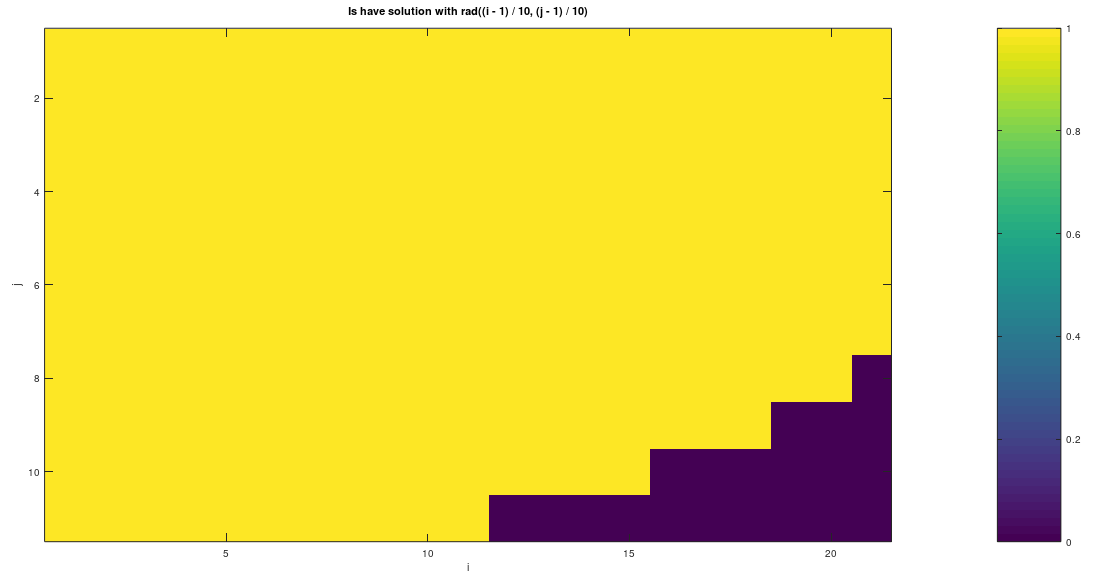
\includegraphics[width=16cm, height=12cm]{solution_map.png}
    \caption{Индикатор наличия решений при заданных радиуасах}
    \label{solve}
\end{figure}
Видим, что здесь у нас потенциально несколько подходящих для продолжения работы комбинаций радиусов. Здесь можно в силу оговоренных в начале обстоятельств воспользоваться той же метрикой (\ref{metric}) для транспонированных нижних строк новой и исходной матрицы $\textbf{A}$.
\\Новые радиусы: [0.6 2]
\\Расстояние по метрике: 0.28
\\Новая матрица: $\textbf{A}_{opt} = \begin{pmatrix}
        [3;4]& [5;6]\\
        [-0.6;0.6]& [-3;1]
        \end{pmatrix}$
\\Решение: $\textbf{x} = \begin{pmatrix}
        [0.05;0.71]\\
        [-0.52;0.19]
        \end{pmatrix}$
\\Итераций: 3
\\Погрешность (порядок): $10^{-16}$
\\В силу малого числа итераций представим матрицу субградиента D и вектор разности dx на каждой итерации:
\\$\textrm{D}^{(1)} = \begin{pmatrix}
        3& 6& 0& 0\\
        0& 0& 0& -3\\
        0& 0& 3& 6\\
        0& -3& 0& 0
        \end{pmatrix}$, $\textrm{dx}^{(1)} = \begin{pmatrix}
        -1.95&\\
        1.33&\\
        1.10&\\
        -0.67&
        \end{pmatrix}$
\\$\textrm{D}^{(2)} = \begin{pmatrix}
        3& 6& 0& 0\\
        0& 0& -0.6& -3\\
        0& 0& 4& 6\\
        0& -3& 0.6& 0
        \end{pmatrix}$, $\textrm{dx}^{(2)} = \begin{pmatrix}
        -0.29&\\
        0.14&\\
        0.05&\\
        -0.14&
        \end{pmatrix}$
\\$\textrm{D}^{(3)} = \begin{pmatrix}
        3& 6& 0& 0\\
        0& 1& -0.6& -3\\
        0& 0& 4& 6\\
        0& -3& 0.6& 0
        \end{pmatrix}$, $\textrm{dx}^{(3)} = \begin{pmatrix}
        -0.0&\\
        0.0&\\
        0.0&\\
        -0.0&
        \end{pmatrix}$
\\Видим, что второй интервал остался без изменений. Значит, уточнять нужно только первый.
\\Составим карту-индикатор наличия решений при растягивании интервала [-0.6;0.6] в разные стороны:
\begin{figure}[H]
    \centering
    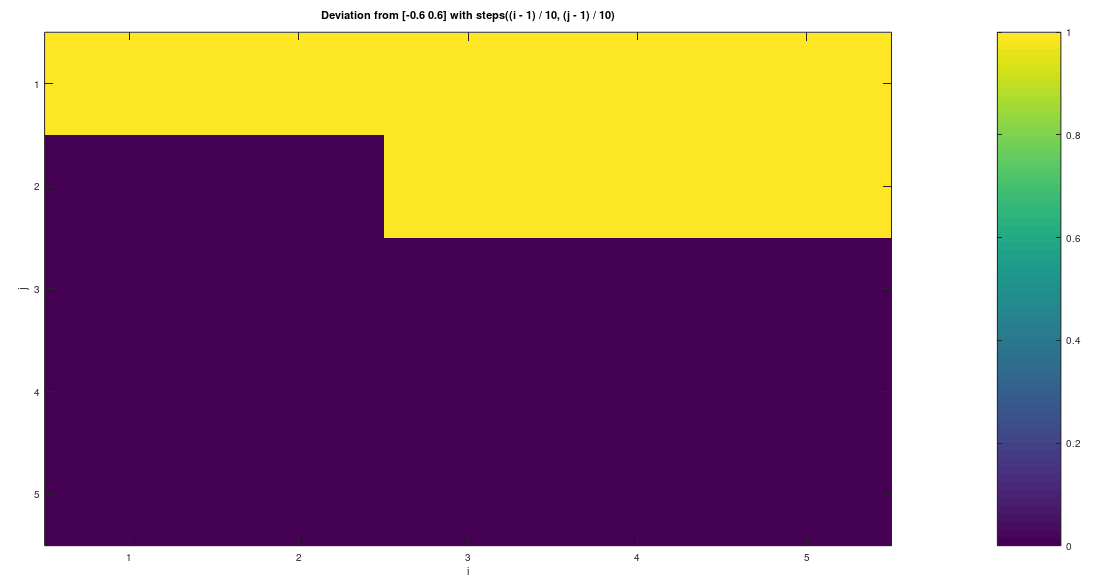
\includegraphics[width=16cm, height=12cm]{dev_from_06.png}
    \caption{Индикатор решений при отклонении от [-0.6;0.6]}
    \label{solve_06}
\end{figure}
Очевидно, что отклонение 0.1 влево и 0.4 вправо является оптимальным на данной сетке. Получим новую матрицу: $\textbf{A}_{opt} = \begin{pmatrix}
        [3;4]& [5;6]\\
        [-0.7;1]& [-3;1]
        \end{pmatrix}$
Таким образом, различия от исходной матрицы проявляются лишь в нижней границе левого нижнего интервала. Но даже ее можно немного улучшить до -0.75. При этом для -0.751 и -0.7501 решений уже нет. В итоге получили:
\\Расстояние по метрике: 0.125
\\Новая матрица: $\textbf{A}_{opt} = \begin{pmatrix}
        [3;4]& [5;6]\\
        [-0.75;1]& [-3;1]
        \end{pmatrix}$
\\Решение: $\textbf{x} = \begin{pmatrix}
        [-0.15;0.8]\\
        [-0.4;0.13]
        \end{pmatrix}$
\\Итераций: 4
\\Погрешность: 0
\\В силу малого числа итераций представим матрицу субградиента D и вектор разности dx на каждой итерации:
\\$\textrm{D}^{(1)} = \begin{pmatrix}
        3& 6& 0& 0\\
        0& 0& 0& -3\\
        0& 0& 3& 6\\
        0& -3& 0& 0
        \end{pmatrix}$, $\textrm{dx}^{(1)} = \begin{pmatrix}
        -2.13&\\
        1.44&\\
        1.57&\\
        -0.97&
        \end{pmatrix}$
\\$\textrm{D}^{(2)} = \begin{pmatrix}
        3& 6& 0& 0\\
        0& 0& -0.75& -3\\
        0& 0& 4& 6\\
        0& -3& 1& 0
        \end{pmatrix}$, $\textrm{dx}^{(2)} = \begin{pmatrix}
        -0.53&\\
        0.27&\\
        0.13&\\
        -0.2&
        \end{pmatrix}$
\\$\textrm{D}^{(3)} = \begin{pmatrix}
        4& 6& 0& 0\\
        0& 1& -0.75& -3\\
        0& 0& 4& 6\\
        0& -3& 1& 0
        \end{pmatrix}$, $\textrm{dx}^{(3)} = \begin{pmatrix}
        0.05&\\
        0.0&\\
        0.0&\\
        -0.0&
        \end{pmatrix}$
\\$\textrm{D}^{(4)} = \begin{pmatrix}
        4& 6& 0& 0\\
        0& 1& -0.75& 0\\
        0& 0& 4& 6\\
        0& -3& 1& 0
        \end{pmatrix}$, $\textrm{dx}^{(4)} = \begin{pmatrix}
        -0.0&\\
        0.0&\\
        0.0&\\
        -0.0&
        \end{pmatrix}$
\subsection{Вывод}
Можно заключить, что рассмотренная в данной работе эвристика справилась с поиском границ наличия решения. При этом интересным оказывается факт, что относительно небольшое смещение лишь одного из интервалов исходной системы привело ее к разрешимости. При решении ИСЛАУ субдифференциальным методом Ньютона сложно сказать, из-за чего могли возникнуть с исходной системой. Ведь были получены целые полосы радиусов, при которых решения существуют. Возможно, это связано с тем, что при вычислении субградиента имеется 16 различных случаев, в зависимости от которых матрица субградиента заполняется тем или иным способом в зависимости от принадлежности интервалов матрицы и приближенного решения к тому или иному типу интервалов, но при этом некоторые случаи разбиваются на подслучаи в зависимости от произведения инфимумов и супремумов этих интервалов. Так же можно заметить общую тенденцию, что по мере приближения наших данных к исходным возрастают абсолютные значения компонент векторов погрешностей dx.
\end{document}